% Options for packages loaded elsewhere
\PassOptionsToPackage{unicode}{hyperref}
\PassOptionsToPackage{hyphens}{url}
%
\documentclass[
]{article}
\usepackage{amsmath,amssymb}
\usepackage{lmodern}
\usepackage{iftex}
\ifPDFTeX
  \usepackage[T1]{fontenc}
  \usepackage[utf8]{inputenc}
  \usepackage{textcomp} % provide euro and other symbols
\else % if luatex or xetex
  \usepackage{unicode-math}
  \defaultfontfeatures{Scale=MatchLowercase}
  \defaultfontfeatures[\rmfamily]{Ligatures=TeX,Scale=1}
  \setmainfont[]{Arial}
\fi
% Use upquote if available, for straight quotes in verbatim environments
\IfFileExists{upquote.sty}{\usepackage{upquote}}{}
\IfFileExists{microtype.sty}{% use microtype if available
  \usepackage[]{microtype}
  \UseMicrotypeSet[protrusion]{basicmath} % disable protrusion for tt fonts
}{}
\makeatletter
\@ifundefined{KOMAClassName}{% if non-KOMA class
  \IfFileExists{parskip.sty}{%
    \usepackage{parskip}
  }{% else
    \setlength{\parindent}{0pt}
    \setlength{\parskip}{6pt plus 2pt minus 1pt}}
}{% if KOMA class
  \KOMAoptions{parskip=half}}
\makeatother
\usepackage{xcolor}
\IfFileExists{xurl.sty}{\usepackage{xurl}}{} % add URL line breaks if available
\IfFileExists{bookmark.sty}{\usepackage{bookmark}}{\usepackage{hyperref}}
\hypersetup{
  pdftitle={Cambodia Biodiversity Paper: Notes on approaches to biodiversity data structure--July 18, 2022},
  hidelinks,
  pdfcreator={LaTeX via pandoc}}
\urlstyle{same} % disable monospaced font for URLs
\usepackage[margin=1in]{geometry}
\usepackage{longtable,booktabs,array}
\usepackage{calc} % for calculating minipage widths
% Correct order of tables after \paragraph or \subparagraph
\usepackage{etoolbox}
\makeatletter
\patchcmd\longtable{\par}{\if@noskipsec\mbox{}\fi\par}{}{}
\makeatother
% Allow footnotes in longtable head/foot
\IfFileExists{footnotehyper.sty}{\usepackage{footnotehyper}}{\usepackage{footnote}}
\makesavenoteenv{longtable}
\usepackage{graphicx}
\makeatletter
\def\maxwidth{\ifdim\Gin@nat@width>\linewidth\linewidth\else\Gin@nat@width\fi}
\def\maxheight{\ifdim\Gin@nat@height>\textheight\textheight\else\Gin@nat@height\fi}
\makeatother
% Scale images if necessary, so that they will not overflow the page
% margins by default, and it is still possible to overwrite the defaults
% using explicit options in \includegraphics[width, height, ...]{}
\setkeys{Gin}{width=\maxwidth,height=\maxheight,keepaspectratio}
% Set default figure placement to htbp
\makeatletter
\def\fps@figure{htbp}
\makeatother
\setlength{\emergencystretch}{3em} % prevent overfull lines
\providecommand{\tightlist}{%
  \setlength{\itemsep}{0pt}\setlength{\parskip}{0pt}}
\setcounter{secnumdepth}{-\maxdimen} % remove section numbering
\ifLuaTeX
  \usepackage{selnolig}  % disable illegal ligatures
\fi

\title{Cambodia Biodiversity Paper: Notes on approaches to biodiversity
data structure--July 18, 2022}
\author{}
\date{\vspace{-2.5em}}

\begin{document}
\maketitle

\textbf{Conceptual notes:}

The biodiversity portfolio (\(B\)) represents the portfolio of fish that
are available in the system that fishers interact with. We don't have
clear system boundaries or a true representation of \(B\), so this file
explores several proxies for \(B\) that could be considered.
\textbf{Each of the aoproaches below makes an assumption about the
system boundaries.} Ideally we would have an observed \(B\) with clearly
defined system boundaries and that contains the full catch portfolio of
fishers (\(C\)), which we directly observe in our sample. You will see
below that this is not the case.

The consumption portfolio (\(M\)) represents the subset of \(C\) that
fishing households consume. We directly observe \(M\) in our data. Due
to the strucutre of the data collection, \(M\) should be fully contained
by \(C\) (though this hasn't been verified in the data just yet).

The notes below demonstrate the issues associated with our observed
\(B\), which I am calling \(\hat{B}\). I show that the species reported
in \(C\) are not strictly contained in \(\hat{B}\) at any level, and
explore various versions of \(\hat{B}\) and the assumptions associated
with each.

\textbf{Available data:}

\begin{enumerate}
\def\labelenumi{\arabic{enumi}.}
\item
  Biomonitoring data was collected at 3-month intervals from November
  2012 until November 2015 for a total of 13 time points. Biomonitoring
  data are repsented in this document by \(\hat{B}\).
\item
  Household catch data was collected at approximately 2-month intervals
  from November 2012 until November 2015 with a total of 19 time points.
  The intervals are disrupted in mid-2013, and throughout the period
  they only partially align with \(\hat{B}\) time points. Catch data are
  observed and therefore represented by \(C\).
\item
  Household consumption data was collected at the same intervals as the
  catch data. Consumption is recorded by species caught rather than a
  standard consumption module. Consumption data are observed and
  therefore represented by \(M\).
\end{enumerate}

Throughout this document \(c\) indexes the CFR associated with the
household and \(i\) indexes the household itself. The time index, \(t\),
represents the observed time points for \(C\) and \(M\), which are
observed at the same times, and \(z\) is the time index for \(\hat{B}\)
(to distinguish from time points \(t\) which do not align with \(z\)).

Here is a schematic of the data structure for reference.

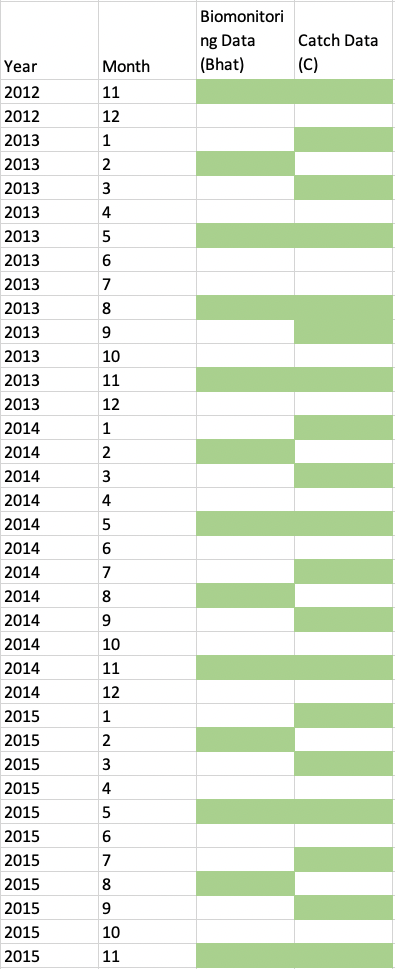
\includegraphics{images/data_structure1.png}

Because the time points for \(C\) and (\(\hat{B}\)) do not line up, we
will have to make \textbf{assumptions about the relationship between
\(B\) and \(C\) over time.} Even if they were aligned in time, some
assumptions would be required, as it is not clear that using a
contemporaneous proxy for \(B\) is the correct approach, given seasonal
dynamics and geographical dispersion of fish beyond the area where the
biomonitoring (\(\hat{B}\)) takes place.

In sum, all of the approaches below vary the assumptions related to
\textbf{system boundaries} and the \textbf{relationship between \(B\)
and \(C\)} over time\\
\strut \\

\hypertarget{approach-1-use-only-contemporaneous-observations-of-hatb-and-c}{%
\subparagraph{\texorpdfstring{\textbf{APPROACH 1: Use only
contemporaneous observations of \(\hat{B}\) and
\(C\)}}{APPROACH 1: Use only contemporaneous observations of \textbackslash hat\{B\} and C}}\label{approach-1-use-only-contemporaneous-observations-of-hatb-and-c}}

\hfill\break
\hfill\break
This approach assumes that the true \(B\) is best represented by
\(\hat{B}\) at the same point in time as \(C\). It assumes that the
system boundary is related to the CFR itself: e.g.~each household is
operating within a system that is somehow associated with the CFR in
their community. This assumption means there are 40 different systems
within the study area that could have different values of \(B\).

No values of \(\hat{B}\) are aggregated across time under this scenario.
The ``timekey3'' variable flags only cases where the year-month align
perfectly between \(\hat{B}\) and (\(C\)) and we merge the data using
this timekey. This is the most conservative and involves dropping
roughly half of catch observations where there is not contemporaneous
\(\hat{B}\).

This can also be expressed as: \(\hat{B}_{ct}^0 = \hat{B}_{cz}\), where
\(t = z\).

When we restrict to only cases where \(t = z\), how often do fishers
catch species that are not found in biomonitoring? Catch \(C\) is
conceptually a subset of \(B\), but in practice may not be fully
contained in \(\hat{B}\), the observed biomonitoring data is limited in
origin to the CFR itself.

In all subsequent tables, ``Matched (N)'' and ``Unmatched (N)'' indicate
the number of cases where a household catches a species that is/isn't
represented in \(\hat{B}\), as defined by each approach. The numbers are
all greater than the total number of households because each household
has at least one catch-species combination in each time point (assuming
they fished in that time point).

\begin{longtable}[]{@{}llll@{}}
\caption{Table 1: Contemporaneous (approach 1)}\tabularnewline
\toprule
Time Period & Unmatched (N) & Matched (N) & Unmatched (\%) \\
\midrule
\endfirsthead
\toprule
Time Period & Unmatched (N) & Matched (N) & Unmatched (\%) \\
\midrule
\endhead
1 & 741 & 426 & 63 \\
2 & 260 & 137 & 65 \\
3 & 628 & 235 & 73 \\
4 & 624 & 410 & 60 \\
5 & 284 & 159 & 64 \\
6 & 394 & 298 & 57 \\
7 & 195 & 143 & 58 \\
8 & 313 & 229 & 58 \\
\bottomrule
\end{longtable}

As shown in Table 1, there are many many cases where species are caught
by fishers that were not found in the contemporaneous biomonitoring data
\(\hat{B}_{ct}^0\) (between 57-73\% of all cases). One way of thinking
about this is that \(C\) is a ``sample'' of the biodiversity porfolio
\(B\), albeit not a random one, taken many more times and in a different
set of locations than \(\hat{B}\) data collection in a given period. The
fish catch data is the list of species from the prior week's catch by
approximately 10 households per CFR, so is not surprising that these
fishers a wider range of species. Furthermore, the fishers are fishing
beyond the borders of the CFR, therefore the spatial area in which they
``sample'' is more diverse. (In fact, I think fishing within the CFR is
normally prohibited, so they are explicitly NOT fishing in the CFR,
though the degree to which other water bodies are connected to the CFR
varies widely by CFR type, location, and season).\\
\strut \\

\hypertarget{approach-2-time-bound-sum-of-lagged-observation-of-b}{%
\subparagraph{\texorpdfstring{\textbf{APPROACH 2: Time-bound sum of
lagged observation of
\(B\)}}{APPROACH 2: Time-bound sum of lagged observation of B}}\label{approach-2-time-bound-sum-of-lagged-observation-of-b}}

\hfill\break
\hfill\break
This approach maintains the system boundary assumption from Approach 1,
that the system boundary is related to the CFR itself and there are 40
different systems with different \(B\)s. Approach 2 makes a different
assumption about the relationship over time between \(\hat{B}\) and
\(C\).

We can imagine that the species richness of the fishery beyond the CFR
is influenced by species richness in the CFR over a longer period of
time: For example, some fish species found in a CFR at a given time
point \(t\) may migrate and be caught by fishers elsewhere at a later
time point \(t+x\), but no longer show up in CFR monitoring at \(t+x\).
In this case, contemporaneous observation does not accurately depict the
biodiversity in the system.

To address this scenario, potential proxies for \(B\) could involve
aggregating values of \(\hat{B}\) over a given number of time periods,
\(x\), with \(x\) ranging from 2 to 13. For a given time period t, the
value of \(\hat{B}\) would be the sum of \(\hat{B}\) over \(x\) time
periods preceding \(t\). The time periods would then be ``rolling,'' and
\(x\) initial observations of \(C\) would be dropped depending on the
value of \(x\). Thus, there is a tradeoff to aggregation if we impose
strict temporal limits, requiring that values of \(\hat{B}\) applied to
values of \(C\) must be aggregated across periods \emph{during or prior}
to t, but not periods \emph{after}). The more time we aggregate across,
the more early catch data we lose. We also potentially lose variation in
\(\hat{B}\).

Example, where x = 2:
\(\hat{B}_{ct}^1 = \hat{B}_{cz} + \hat{B}_{c,z-1}\)

Here is an image in case my notation is a failure.

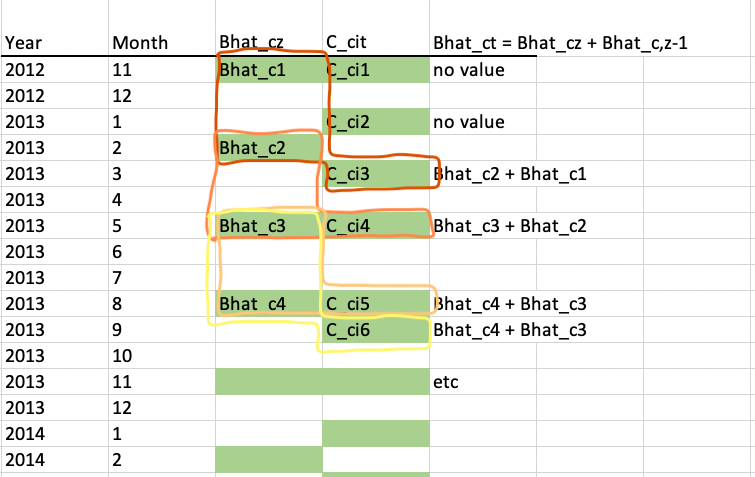
\includegraphics{images/data_structure2.png}

Table 2 shows the percentage of species found in household catch that is
not found in \(hat{B}_{ct}^1\) as defined above. The same data broken
down by CFR shows similar percentages. Though lower than the
contemporaneous scenario, they are still quite high, ranging from 29-52
percent.

\begin{longtable}[]{@{}llll@{}}
\caption{Time-bound sum of Bhat (approach 2)}\tabularnewline
\toprule
Time Period & Unmatched (N) & Matched (N) & Unmatched (\%) \\
\midrule
\endfirsthead
\toprule
Time Period & Unmatched (N) & Matched (N) & Unmatched (\%) \\
\midrule
\endhead
3 & 269 & 408 & 40 \\
4 & 205 & 285 & 42 \\
5 & 495 & 476 & 51 \\
6 & 526 & 491 & 52 \\
7 & 550 & 640 & 46 \\
8 & 356 & 496 & 42 \\
9 & 223 & 508 & 31 \\
10 & 201 & 366 & 35 \\
11 & 255 & 448 & 36 \\
12 & 313 & 423 & 43 \\
13 & 324 & 507 & 39 \\
14 & 198 & 347 & 36 \\
15 & 156 & 373 & 29 \\
16 & 148 & 303 & 33 \\
17 & 193 & 331 & 37 \\
18 & 326 & 364 & 47 \\
19 & 284 & 386 & 42 \\
\bottomrule
\end{longtable}

\hfill\break
\hfill\break

\hypertarget{approach-3-apply-the-sum-of-total-species-richness-across-time-by-cfr-to-each-catch-time-point.}{%
\subparagraph{\texorpdfstring{\textbf{APPROACH 3: Apply the sum of total
species richness across time by CFR to each catch time
point.}}{APPROACH 3: Apply the sum of total species richness across time by CFR to each catch time point.}}\label{approach-3-apply-the-sum-of-total-species-richness-across-time-by-cfr-to-each-catch-time-point.}}

\hfill\break
\hfill\break
Another option is to eliminate the strict temporal limits described
above and allow \(B\) to include species identified in time points
\emph{after} we observe \(C\). One version of this is to apply the total
species richness across the entire study period for a given CFR to each
catch time point, thus maintaining the assumption that the CFR is
related to the system boundary. This reduces the temporal variation in
\(\hat{B}\), but there is still variation across CFRs. This assumption
also obscures variation in \(B\) over time that might be relevant, such
as seasonal variation and time trends.

This would be expressed as:
\(\hat{B}_{c}^2 = \sum_{t=1}^{13} \hat{B}_{ct}\)

Table 3 demonstrates a much lower percentage unmatched relative to the
previous approaches, ranging from 11-25 percent of cases.

\begin{longtable}[]{@{}llll@{}}
\caption{Sum of Bhat across all time periods, by CFR (approach
3)}\tabularnewline
\toprule
Time Period & Unmatched (N) & Matched (N) & Unmatched (\%) \\
\midrule
\endfirsthead
\toprule
Time Period & Unmatched (N) & Matched (N) & Unmatched (\%) \\
\midrule
\endhead
1 & 295 & 872 & 25 \\
2 & 103 & 529 & 16 \\
3 & 96 & 456 & 17 \\
4 & 52 & 356 & 13 \\
5 & 149 & 714 & 17 \\
6 & 161 & 747 & 18 \\
7 & 229 & 805 & 22 \\
8 & 143 & 581 & 20 \\
9 & 93 & 474 & 16 \\
10 & 70 & 378 & 16 \\
11 & 66 & 489 & 12 \\
12 & 74 & 541 & 12 \\
13 & 108 & 584 & 16 \\
14 & 65 & 383 & 15 \\
15 & 50 & 351 & 12 \\
16 & 38 & 302 & 11 \\
17 & 53 & 349 & 13 \\
18 & 93 & 493 & 16 \\
19 & 89 & 476 & 16 \\
\bottomrule
\end{longtable}

\hfill\break
\hfill\break

\hypertarget{approach-4-apply-the-sum-of-total-species-richness-across-time-and-cfr-to-each-catch-time-point}{%
\subparagraph{\texorpdfstring{\textbf{APPROACH 4: Apply the sum of total
species richness across time and CFR to each catch time
point}}{APPROACH 4: Apply the sum of total species richness across time and CFR to each catch time point}}\label{approach-4-apply-the-sum-of-total-species-richness-across-time-and-cfr-to-each-catch-time-point}}

\hfill\break
\hfill\break
An alternate approach would be to apply the total species richness
across the entire study period and across all CFRs to each catch time
point. This is a more permissive version of the above approach that
eliminates the assumption that the CFR is the relevant system boundary.
It treats the system as singular and each of the households faces the
same set of \(B\) from which to draw their catch.

The practical value here is that it should generate the smallest number
of unmatched cases. Unmatched cases, under this approach, represent
species that were caught by fishers but \emph{never} appeared in
\emph{any} biomonitoring in \emph{any} CFR at \emph{any} time period.

\begin{longtable}[]{@{}llll@{}}
\caption{Sum of Bhat across all time periods and CFRs (approach
4)}\tabularnewline
\toprule
Time Period & Unmatched (N) & Matched (N) & Unmatched (\%) \\
\midrule
\endfirsthead
\toprule
Time Period & Unmatched (N) & Matched (N) & Unmatched (\%) \\
\midrule
\endhead
1 & 11 & 1156 & 1 \\
2 & 2 & 630 & 0 \\
3 & 1 & 551 & 0 \\
4 & 0 & 408 & 0 \\
5 & 0 & 863 & 0 \\
6 & 2 & 906 & 0 \\
7 & 4 & 1030 & 0 \\
8 & 1 & 723 & 0 \\
9 & 0 & 567 & 0 \\
10 & 0 & 448 & 0 \\
11 & 0 & 555 & 0 \\
12 & 1 & 614 & 0 \\
13 & 2 & 690 & 0 \\
14 & 0 & 448 & 0 \\
15 & 0 & 401 & 0 \\
16 & 0 & 340 & 0 \\
17 & 1 & 401 & 0 \\
18 & 0 & 586 & 0 \\
19 & 0 & 565 & 0 \\
\bottomrule
\end{longtable}

Table 4 illustrates that this approach successfully eliminates
mismatches. However, if we want to make the case that households in more
diverse systems are (or are not) accessing more diverse nutrients, the
intuitively we want individual households to be facing some range of
system diversity over space and/or time, rather than holding diversity
constant for all households across space and time. Useful variation in
diversity should be across space (e.g.~in relation to CFRs) or time
(seasonally or ???).\\
\strut \\

\hypertarget{side-investigation-which-fish-species-are-represented-in-c-but-not-in-hatb}{%
\subparagraph{\texorpdfstring{\textbf{Side investigation:} Which fish
species are represented in \(C\) but not in
\(\hat{B}\)?}{Side investigation: Which fish species are represented in C but not in \textbackslash hat\{B\}?}}\label{side-investigation-which-fish-species-are-represented-in-c-but-not-in-hatb}}

\begin{longtable}[]{@{}lll@{}}
\caption{Species that never appear in Bhat}\tabularnewline
\toprule
Species Code & Species Name'' & Occurrences \\
\midrule
\endfirsthead
\toprule
Species Code & Species Name'' & Occurrences \\
\midrule
\endhead
73 & Acantopsis thiemmedhi & 7 \\
80 & Pangio fusca & 12 \\
114 & Cyprinus carpio carpio & 3 \\
144 & Bagarius yarrelli & 3 \\
152 & Tuberoschistura cambodgiensis & 1 \\
\bottomrule
\end{longtable}

\hfill\break
\hfill\break

\hypertarget{approach-5-aggregate-hatb-by-season-month}{%
\subparagraph{\texorpdfstring{\textbf{APPROACH 5: Aggregate \(\hat{B}\)
by season
(month)}}{APPROACH 5: Aggregate \textbackslash hat\{B\} by season (month)}}\label{approach-5-aggregate-hatb-by-season-month}}

\hfill\break
\hfill\break
In order to maintain spatial and temporal variation, but increase the
level of aggregation to something higher than Approach 2 and but lower
than Approach 4, I will try aggregating by month and CFR. I think the
relevant seasons are driven by rainfall patterns, which may vary a bit,
but month is a useful rough proxy for the time being. We have 4
observations per year and we aggregate across years, then merge them
with months that appear in the catch data. This leaves us with 5 time
periods.

\begin{longtable}[]{@{}llll@{}}
\caption{Sum of Bhat by month and by CFR (approach 5)}\tabularnewline
\toprule
Time Period & Unmatched (N) & Matched (N) & Unmatched (\%) \\
\midrule
\endfirsthead
\toprule
Time Period & Unmatched (N) & Matched (N) & Unmatched (\%) \\
\midrule
\endhead
1 & 776 & 2033 & 28 \\
4 & 243 & 464 & 34 \\
5 & 855 & 1106 & 44 \\
7 & 690 & 1918 & 26 \\
10 & 298 & 564 & 35 \\
13 & 419 & 1351 & 24 \\
16 & 185 & 542 & 25 \\
19 & 326 & 1101 & 23 \\
\bottomrule
\end{longtable}

In Table 6, unmatched percentages are still quite high. Not as high as
Approach 2, but still very high.\\
\strut \\

\hypertarget{approach-6-aggregate-hatb-by-cfr-type.}{%
\subparagraph{\texorpdfstring{\textbf{APPROACH 6: Aggregate \(\hat{B}\)
by CFR
type}.}{APPROACH 6: Aggregate \textbackslash hat\{B\} by CFR type.}}\label{approach-6-aggregate-hatb-by-cfr-type.}}

\hfill\break
\hfill\break
This approach keeps the time dimension intact, and aggregates the
\(\hat{B}\) spatially by CFR type. There are 4 types of CFRs, defined
as:

\begin{enumerate}
\def\labelenumi{\arabic{enumi}.}
\tightlist
\item
  Reservoir for irrigation in upland area
\item
  Community pond within agricultural land not prone to flood
\item
  Community pond within agricultural land prone to flood
\item
  Demarcated area in larger water body (Perennial fishing)
\end{enumerate}

We have little information about the categories beyond what is written
above. It is reasonable to think that propensity for flooding, being
upland or being a demarcated area in a larger water body could make a
difference to the nature of the CFR's representation of the system
fishers have access to.

Table 7 shows that this approach successfully minimized mismatches,
while retaining \emph{some} variation across space and time. In effect,
this approach defines the system boundary as something related to the
type of CFR, but not the CFR itself. This is likely correlated with the
surrounding geographical features (elevation, slope, water bodies).

\begin{verbatim}
## [1] 0
\end{verbatim}

\begin{longtable}[]{@{}llll@{}}
\caption{Sum of Bhat by CFR type (approach 6)}\tabularnewline
\toprule
Time Period & Unmatched (N) & Matched (N) & Unmatched (\%) \\
\midrule
\endfirsthead
\toprule
Time Period & Unmatched (N) & Matched (N) & Unmatched (\%) \\
\midrule
\endhead
1 & 47 & 2762 & 2 \\
2 & 10 & 1205 & 1 \\
3 & 6 & 1086 & 1 \\
4 & 4 & 703 & 1 \\
5 & 7 & 1954 & 0 \\
6 & 16 & 2351 & 1 \\
7 & 25 & 2583 & 1 \\
8 & 15 & 1693 & 1 \\
9 & 2 & 1197 & 0 \\
10 & 3 & 863 & 0 \\
11 & 3 & 1044 & 0 \\
12 & 7 & 1321 & 1 \\
13 & 9 & 1761 & 1 \\
14 & 4 & 1114 & 0 \\
15 & 2 & 877 & 0 \\
16 & 1 & 728 & 0 \\
17 & 3 & 782 & 0 \\
18 & 4 & 1315 & 0 \\
19 & 6 & 1421 & 0 \\
\bottomrule
\end{longtable}

I'm stopping here because my brain is tired. Amazing that you read this
far! :)

\end{document}
